\documentclass[a4paper, 8pt, twocolumn]{article}
\usepackage{titlesec}					%custom \title \section \subsection 
\usepackage[a4paper, top=1cm, bottom=1cm, left=1cm, right=1cm]{geometry}
\usepackage{amsmath}
\usepackage{graphicx}                   %for Images
\usepackage{enumitem}                  %for itemize

% \usepackage{fontspec} 					%for loading fonts
% \usepackage{xunicode,xltxtra,url,parskip} 	%other packages for formatting
% \RequirePackage{color,graphicx}
% \usepackage[usenames,dvipsnames]{xcolor}
%\usepackage[big]{layaureo} 				%better formatting of the A4 page
% an alternative to Layaureo can be ** \usepackage{fullpage} **
% \usepackage{supertabular} 				%for Grades

%Setup hyperref package, and colours for links
% \usepackage{hyperref}

% customize section text
\titleformat{\section}                  % command to modify
  {\large\bfseries}                     % format applied to label+text
  {}                                    % label (there is none!)
  {0em}                                 % horizontal separation between label and title body
  {}                                    % before the title body
[]                                      % after the title body


\titleformat{\subsection}                  % command to modify
  {\normalsize\bfseries}                     % format applied to label+text
  {}                                    % label (there is none!)
  {0em}                                 % horizontal separation between label and title body
  {}                                    % before the title body
[]                                      % after the title body

\renewcommand{\thesection}{}            % Remove section numbering


\title{Marketing Mix Models}

\begin{document}
\maketitle

\small
\section{Introduction}
 
MMM aims to quantify the impact of marketing activities on sales.
It is a statistical analysis of sales and marketing data to estimate the impact of various marketing tactics on sales.
It helps businesses make judicious decisions, like on which marketing channel to spend and, more importantly, what amount 
should be spent. Reallocate the budget across marketing channels to maximize the return on investment (ROI)

Marketing Mix Modeling has the advantage over a attribution model that it works in the cookieless world that we are heanding
into.

In the end we want to be able to answer questions such as 
\textit{How much of the x amouth of sales in a specific week was generated by tv advertising?
    Ans how much by radio and web banners? And what is the baseline, i.e. the number of sales we 
    would have had without any advertising'}

\small
\section{RoAS (Return on Advertising Spend)}

Its defined as the revenue from an ad campaign divided by the cost of the campaign (multiplied by 100 to get a percentage).
In simple words, ROAS represents the revenue gained from each dollar spent on advertising.

\begin{equation}
    \text{ROAS} = \frac{\text{Revenue}}{\text{Cost}} * 100
\end{equation}

\section{Advertising Adstock}
The term adstock encapsulates two important concepts:
\begin{itemize}[noitemsep]
    \item Carryover, or Lagged  Effect.
    \item Diminishing Returns, or Saturation Effect.
\end{itemize}

\small
\subsection{-> Carryover Effect, or Lagged Effect}
Advertising tends to have an effect extending several periods after you see it for the first time.
An advertisement from erlier day, week, etc. may effect an ad in the current day, week, etc. 

The answer that we need to figure out is \textit{how to include this time period of the delayed impacts of ad in our caluclations?}
The industry answer is something called ADSTOCK - the measure of carry-over and lag effect of marketing activities!.

\small
\subsection{-> Diminishing Returns Effect/Saturation Effect}
Exposure to an advertisement creates awareness about the product in consumers' mind to a certain limit, but after that impact of 
advertisements to inluence consumers' purchasing behavior start diminishing over time. This is called the saturation effect or 
Diminishing Returns Effect.

Simply put, It'd be presumtuous to say that the more money you spend on advertising, the higher your sales get. In reality, 
this growth gets weaker the more we spend.

\begin{figure}[h] % the [h] ensures that the figure is placed here, not at the top/bottom of the page
    \centering
    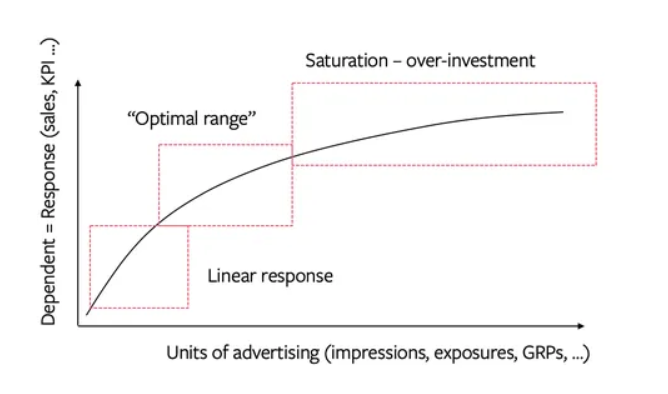
\includegraphics[width=0.35\textwidth]{images/image__diminishing_returns.png} % adjust the width as needed
    \label{fig:example-image}
\end{figure}


\begin{thebibliography}{9}

\bibitem{webpage_robyn} 
\textit{Introduction to Market Mix Models using Robyn}. 
URL: \texttt{https://www.analyticsvidhya.com/blog/2023/05/introduction-to-market-mix-model-using-robyn/}, Accessed: September 11, 2023.
\end{thebibliography}

\bibitem{webpage_vidtao} 
\textit{The measure of carry-over and lag effect of marketing activities - Marketing Mix Modeling (mmm) part 3}. 
URL: \texttt{https://vidtao.com/the-measure-of-carry-over-and-lag-effect-of-marketing-activities-marketing-mix-modeling-mmm-part-3/}, Accessed: September 13, 2023.
\end{thebibliography}


\end{document}
